\chapter{General overview}
\newpage
\section*{Introduction}
This chapter will give you a general overview about the project. We start by presenting the project and analyse the requirements.
\addcontentsline{toc}{section}{Introduction}
\section{Presenting the company}
This project is built for the company VIPAY SARL. I'm one of the interns in the company and
my mission was to build an instructor dashboard for study.tn, an online video based e-learning platform for Tunisia where students can enroll in video based courses, and learn from the best instructors, in their own pace, anywhere, at anytime and in low cost.
\section{Presenting the project}
Study.tn is an e-learning platform : It is a training/education approach that theoretically allows learning without the presence of a physical teacher nearby, 
\hfill \break
\hfill \break
The platform consists of three spaces :

\begin{itemize}
  \item The Student space where students can enroll and watch courses.
  \item The instructor space where the instructor can manage his courses, sales.
  \item The admin space where Study.tn team can manage users and courses 
\end{itemize}

In this project we will build a new instructor dashboard. In this dashboard the instructor can manage the courses, manage sales and communicate with students.
\section{The existing solutions}
\subsection{Analysis of the existing solutions}
The current study.tn website already has its own instructor dashboard where the instructor can add, delete or edit courses. The instructor can set the general informations such as course title,
sub-title, price, description , category and cover photo. They can add chapters and lectures. Instructors can add requirements and exam questions. They can also check their sales.

\begin{figure}[!ht]
    \centering
    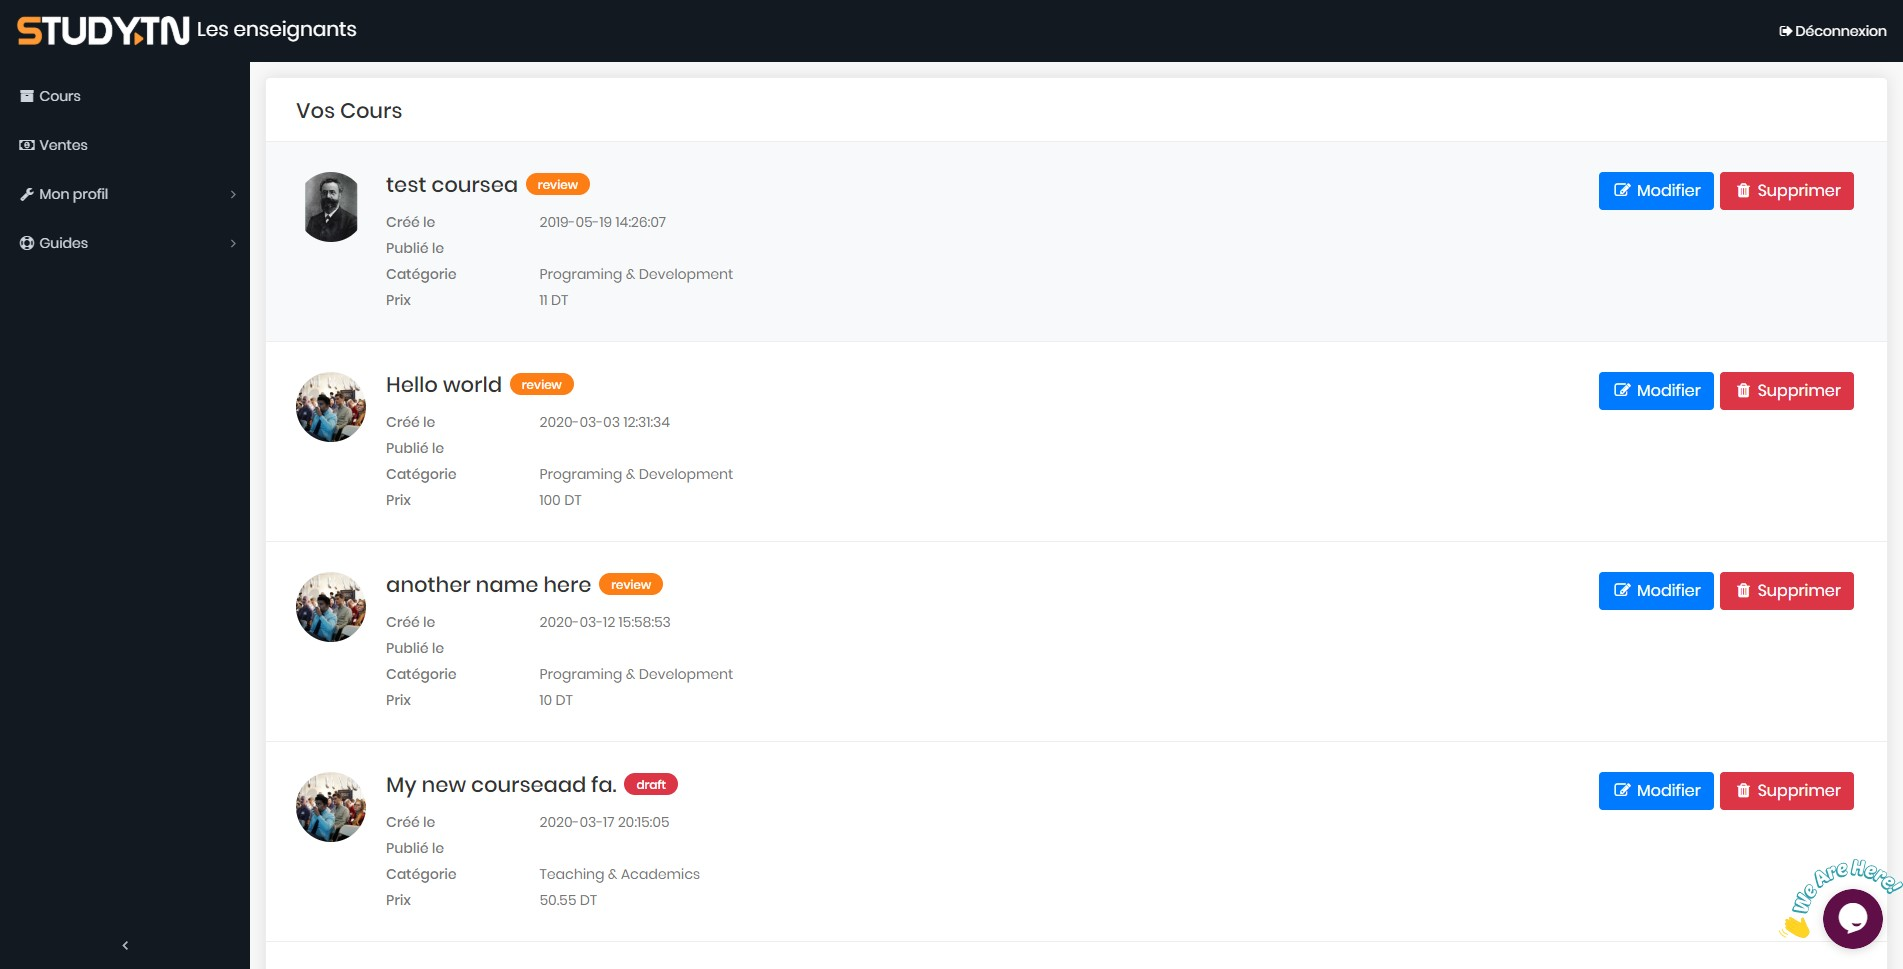
\includegraphics[width=150mm]{currrent_instuctor_space.jpg}
    \caption{The current study.tn instructor dashboard}
    \label{fig:currrent_instuctor_space}
\end{figure}

\subsection{Problem of the existing solutions}
Server-side rendering is a common method for displaying information onto the screen. It works by converting HTML files in the server into usable information for the browser. Whenever you visit a website, your browser makes a request to the server that contains the contents of the website. Once the request is done, your browser will display the rendered HTML on the screen. The current instructor dashboard uses server-side rendering with a template engine which leads to the following issues : 
\begin{itemize}
  \item Touching the front-end risks touching back-end as in theory you can't do a UI rebuild without messing backend.
  \item Full page reloads when changing routes.
  \item Frequent server requests which will increase the load on the server.
  \item An overall slow page rendering as the HTML doc gets bigger.

\end{itemize}

\subsection{Proposed solution}
All of the issues above can be overcomed using a front-end framework. We decided to go with react as it is the most used framework for building large scale web applications. Built by Facebook, React makes it simple to create interactive user interfaces. The framework is designed for building component based applications and with the support of backward compatibility, so you can rest assured of its longevity. React has almost 3 million users and a massive developer community. These are the advantages of using react :


\begin{itemize}
  \item Does not require page reloading during use.
  \item Only load the data from the server when needed.
  \item Fast page rendering as it only re-render the components that needs to be updated.
\end{itemize}


%fin code item
\section{Project management}

\subsection{Agile method}
An Agile method is carried out in a collaborative spirit and adapt to incremental approaches. It generates high-quality products while taking into account requirement changes. It also allows
to manage quality continuously and detect problems as soon as possible,
thus allowing corrective actions to be taken without too many penalties in the
costs and deadlines. For our project, we focused on an
Agile type method and more particularly SCRUM\cite{cite0}.

\subsection{Why SCRUM}
SCRUM is a project management method that only presents qualities: 

\begin{itemize}
  \item It is mainly focused on quality, objectives, efficiency.
  \item Minimization of bugs while allowing an excellent communication in the project through the daily Scrum meeting.
  \item The tasks and the "reviewing" process in the project are perfectly defined which totally improves progress.
\end{itemize}


\vfill
\clearpage

\begin{figure}[!ht]
    \centering
    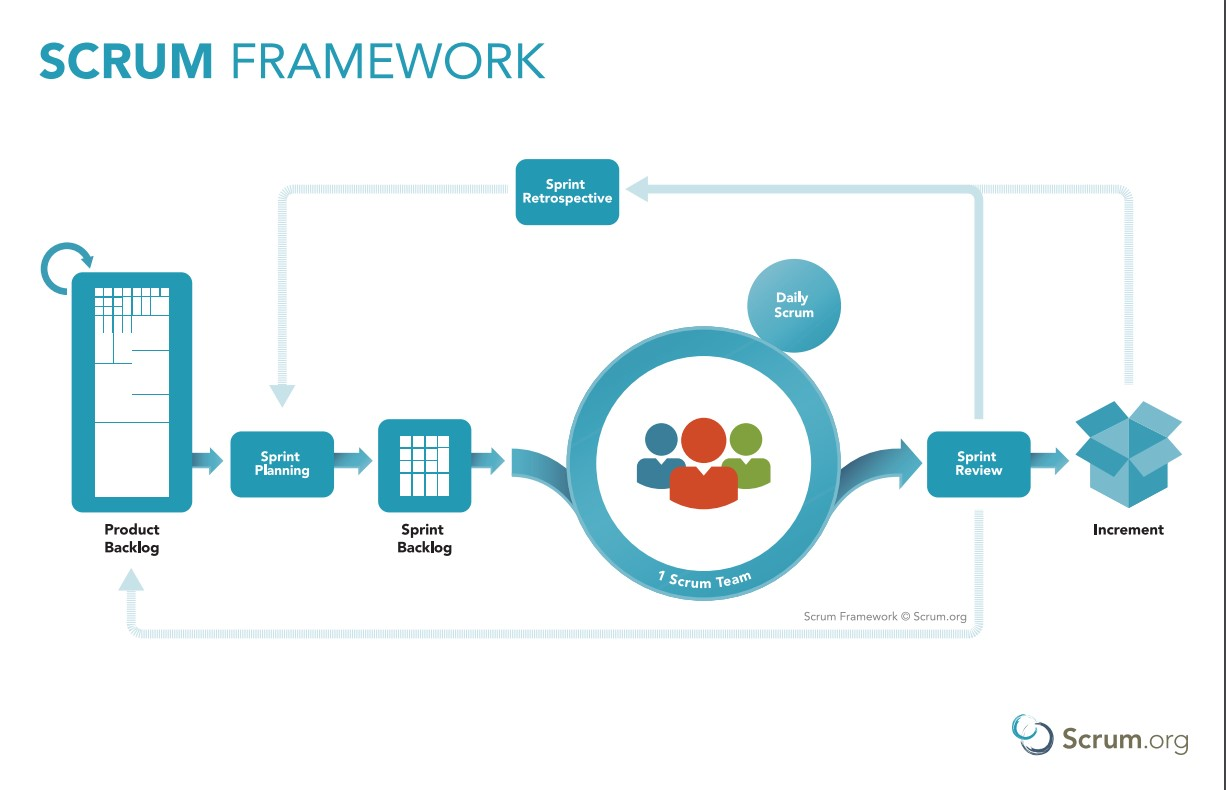
\includegraphics[width=150mm]{scrum.jpg}
    \caption{The Scrum Framework}
    \label{fig:scrum}
\end{figure}



\subsection{UML\cite{cite1}}

UML (Unified Modeling Language) is a formal language normalized in terms of
object modeling.

\subsection{Why UML}
UML brings many advantages such as :
\begin{itemize}
  \item Its independence from programming languages, application and process areas, its versatility and flexibility have made him a universal language.
  \item Make the representation and understanding of object solutions easier.
  \item Its graphic notation allows to express an object solution visually, which helps in the comparison and evaluation of solutions.
\end{itemize}

\section*{Conclusion}
Throughout this chapter, we gave a general overview about the project and we have
presented the existing solution, and the problems in it. We also introduced the company, the work required, and
the chosen methodology. The next chapter will be for the requirements analysis.
